\section{The Area of Work}
Our area of work will specifically be directed towards analyzing and extracting data. We'll be focusing on finding patterns are relation of phrases and words towards positive or negative sentiments of online comments, posts and tweets of the individual.
 

\section{Problem Overview}
The recent boom of online social media creates a giant void of making content be meaningful, to machines along with humans. Social Media giants like Facebook, Twitter, Instagram, Reddit etc. all need this data analyzed to filter out inappropriate content, categorization of posts along with numerous other applications. 
This gap between Hundreds of Terabytes of unrecognized data can be understood using Natural Language Processing, and for the specific problem we discussed, Sentimental Data Analysis hits the key goal.

\section{Solution}
All of the data for the sentiment analysis that we will be using, will be compilation of open source data acquired from product reviews, tweets, blog posts or other social media outlets. Sentiment Analysis can be considered a classification process, There are three main classification levels in Sentiment Analysis: document-level, sentence-level, and aspect-level. We will focus our attention on Sentence-Level sentiment polarity classification.\newline

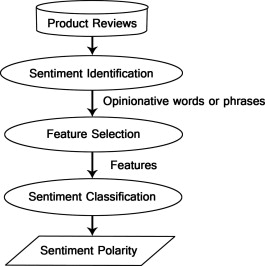
\includegraphics[scale=1]{sentimental-analysis.jpg}\newline
\textsubscript{Source: https://www.sciencedirect.com/science/article/pii/S2090447914000550}


\section{Process}
The process for sentiment analysis varies as the data varies. Only Lexicon based Approach doesn't define a well fitted line for positive and negative sentiment, but helps significantly in associating words with sentiments. To get a well fitted line, we'll focus our approach towards Linear Classifiers. From the empirical comparison between SVMs and Artificial neural networks presented by Moraes and Valiati \cite{moraes2013document}, indicated that ANN produced superior results to SVM except for some unbalanced data contexts. Therefore, we pursue our study in Neural Networks by using labelled data for our Supervised Learning. Neural Network's classification can always be improved by feeding more data.\newline

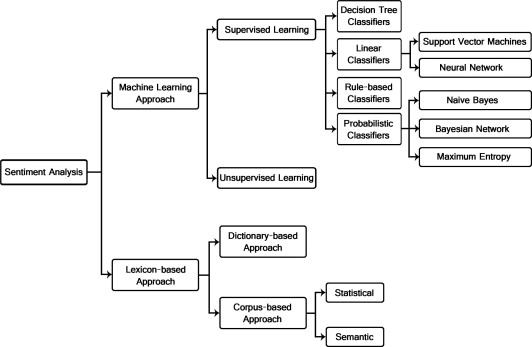
\includegraphics[scale=1]{solution-tree.jpg}\newline
\textsubscript{Source: https://www.sciencedirect.com/science/article/pii/S2090447914000550}

\section{Existing System}
Following sub-sections give brief overview of current systems to tackle Sentiment Analysis. Some of the following summaries are extracted from Sciencedirect's excellent overview of Sentiment Analysis and it's approaches.


\subsection{Machine Learning Approach}
Machine learning approach relies on Machine Learning algorithms to solve the Sentiment Analysis as a regular text classification problem that makes use of syntactic and/or linguistic features.

\subsubsection{Support Vector Machines}
Chen and Tseng \cite{chen2011quality} have used two multiclass SVM-based approaches: One-versus-All SVM and Single-Machine Multiclass SVM to categorize reviews. They proposed a method for evaluating the quality of information in product reviews considering it as a classification problem. They worked on digital cameras and MP3 reviews.

SVMs were used by Li and Li \cite{li2013deriving} as a sentiment polarity classifier. Unlike the binary classification problem, they argued that opinion subjectivity and expresser's credibility should also be taken into consideration. They proposed a framework that provides a compact numeric summarization of opinions on micro-blogs platforms. They identified and extracted the topics mentioned in the opinions associated with the queries of users, and then classified the opinions using SVM. They worked on twitter posts for their experiment.

\subsubsection{Naive Bayes}
The Naïve Bayes classifier is the simplest and most commonly used classifier. Naïve Bayes classification model computes the posterior probability of a class, based on the distribution of the words in the document. The model works with the BOWs feature extraction which ignores the position of the word in the document. It uses Bayes Theorem to predict the probability that a given feature set belongs to a particular label.

$$ P(Label \mid Features) = \frac{P(Features \mid Label) \, P(Label)}{P(Features)} $$

 A better solution was proposed by Kang and Yoo \cite{kang2012senti} to solve the problem of the tendency for the positive classification accuracy to appear up to approximately 10\% higher than the negative classification accuracy. This creates a problem of decreasing the average accuracy when the accuracies of the two classes are expressed as an average value. They showed that using this algorithm with restaurant reviews narrowed the gap between the positive accuracy and the negative accuracy compared to Naive Bayes and SVM.

\subsubsection{Neural Networks}
There is an empirical comparison between Support Vector Machines and Artificial Neural Networks presented by Moraes and Valiati \cite{moraes2013document} regarding document-level sentiment analysis. Their experiments indicated that ANN produced superior results to SVM except for some unbalanced data contexts. They have tested three benchmark data sets on Movie, GPS, Camera and Books Reviews from amazon.com. They proved that the experiments on movie reviews ANN outperformed SVM by a statistically significant difference.

Van de Camp and Van den Bosch's \cite{van2012socialist} case study was based on historical biographical information describing people in a particular domain, region and time frame. They showed that their classifiers were able to label these relations above a majority class baseline score. They found that a training set containing relations, surrounding multiple persons, produces more desirable results than a set that focuses on one specific entity. 


\subsection{Lexicon-based Approach}
Classification using existing positive and negatively defined opinion words.

\subsubsection{Dictionary-based Approach}
\cite{hu2004mining} and \cite{kim2004determining} presented the main strategy of the dictionary-based approach. A small set of opinion words is collected manually with known orientations. Then, this set is grown by searching in the well known corpora WordNet \cite{miller1990introduction} or thesaurus \cite{mohammad2009generating} for their synonyms and antonyms. The newly found words are added to the seed list then the next iteration starts. The iterative process stops when no new words are found. After the process is completed, manual inspection can be carried out to remove or correct errors.

Qiu and He \cite{qiu2010dasa} used dictionary-based approach to identify sentiment sentences in contextual advertising. They proposed an advertising strategy to improve ad relevance and user experience. They used syntactic parsing and sentiment dictionary and proposed a rule based approach to tackle topic word extraction and consumers’ attitude identification in advertising keyword extraction. They worked on web forums from automotvieforums.com. 



\subsubsection{Statistical Analysis}
Finding co-occurrence patterns or seed opinion words can be done using statistical techniques. This could be done by deriving posterior polarities using the co-occurrence of adjectives in a corpus, as proposed by Fahrni and Klenner \cite{fahrni2008old}.
The polarity of a word can be identified by studying the occurrence frequency of the word in a large annotated corpus of texts \cite{read2009weakly}. If the word occurs more frequently among positive texts, then its polarity is positive. If it occurs more frequently among negative texts, then its polarity is negative. If it has equal frequencies, then it is a neutral word.

Hu and Bose \cite{hu2012manipulation} expected that the writing style of the reviews would be random due to the various backgrounds of the customers, if the reviews were written actually by customers. They worked on Book reviews from amazon.com and discovered that around 10.3\% of the products are subject to online reviews manipulation.

Latent Semantic Analysis (LSA) is a statistical approach which is used to analyze the relationships between a set of documents and the terms mentioned in these documents in order to produce a set of meaningful patterns related to the documents and terms \cite{deerwester1990indexing}. Cao and Duan \cite{cao2011exploring} have used LSA to find the semantic characteristics from review texts to examine the impact of the various features. The objective of their work is to understand why some reviews receive many helpfulness votes, while others receive few or no votes at all. They investigated the factors that determine the number of helpfulness votes which a particular review receives (include both “yes” and “no” votes). They worked on software programs users’ feedback from CNET Download.com. They showed that the semantic characteristics are more influential than other characteristics in affecting how many helpfulness vote reviews receive.


\subsubsection{Semantic Analysis}
The Semantic approach gives sentiment values directly and relies on different principles for computing the similarity between words. This principle gives similar sentiment values to semantically close words.

The Semantic approach is used in many applications to build a lexicon model for the description of verbs, nouns and adjectives to be used in SA as the work presented by Maks and Vossen \cite{maks2012lexicon}. Their model described the detailed subjectivity relations among the actors in a sentence expressing separate attitudes for each actor. These subjectivity relations are labeled with information concerning both the identity of the attitude holder and the orientation (positive vs. negative) of the attitude. It provided means for the identification of the attitude holder, the polarity of the attitude and also the description of the emotions and sentiments of the different actors involved in the text. They used Dutch WordNet in their work. Their results showed that the speaker’s subjectivity and sometimes the actor’s subjectivity can be reliably identified.


\section{Our Approach}
Support Vector Machines and Neural Networks can be used also for the classification of personal relationships in biographical texts as presented by van de Camp and van den Bosch \cite{van2012socialist}. They marked relations between two persons as positive, neutral, or unknown. They showed that their classifiers were able to label these relations above a majority class baseline score. They found that a training set containing relations, surrounding multiple persons, produces more desirable results than a set that focuses on one specific entity. They proved that SVM and one layer NN (1-NN) algorithm achieve the highest scores.
In order to get more relevant intelligence and better efficiency we strive to achieve, we pursued towards more of a generalized solution than one that will only work on a specific dataset.\newline
Considering all the available approaches, we chose to go with the most sustainable, expandable and efficient way. Hence, to find the best combination, we selected the Lexicon Based approach, along with Neural Networks, coherent with the dataset.